%%%%%%%%%%%%%%%%%%%%%%%%%%%%%%%%%%%%%%%%%%%%%%%%%%%%%%%%%%%%%%%%%%%%%%%%%%%%%%%

\chapter{FERRAMENTA LOMB-SCARGLE}

O periodograma de Lomb-Scargle é a ferramenta padrão para dados com sampling rates não uniformes. Dito isto, é muito importante a compreensão dos diferentes artefatos presentes na análise espectral e a diferenciação de suas origens. 

\section{Efeitos da amostragem}

Os principais artefatos da análise espctral são o \textit{aliasing} e o \textit{spectral leakage}. Leakage espectral é o ``vazamento'' da energia devida a uma frequência existente no sinal para outras, por exemplo os lóbulos laterais presentes em muitos espectros. Aliasing é um tipo de leakage, que é o efeito do espectro apresentar assinaturas falsas de sinais (alias vem do inglês e significa pseudônimo). As Figuras \ref{fig:window} e \ref{fig:sampling} exemplificam tais fenômenos e ilustram suas causas.

\begin{figure}[ht!]
	\caption{Efeitos da amostragem finita.}
	\vspace{1mm}	% acrescentar o espaçamento vertical apropriado entre o título e a borda superior da figura
	\begin{center}
		\resizebox{15cm}{!}{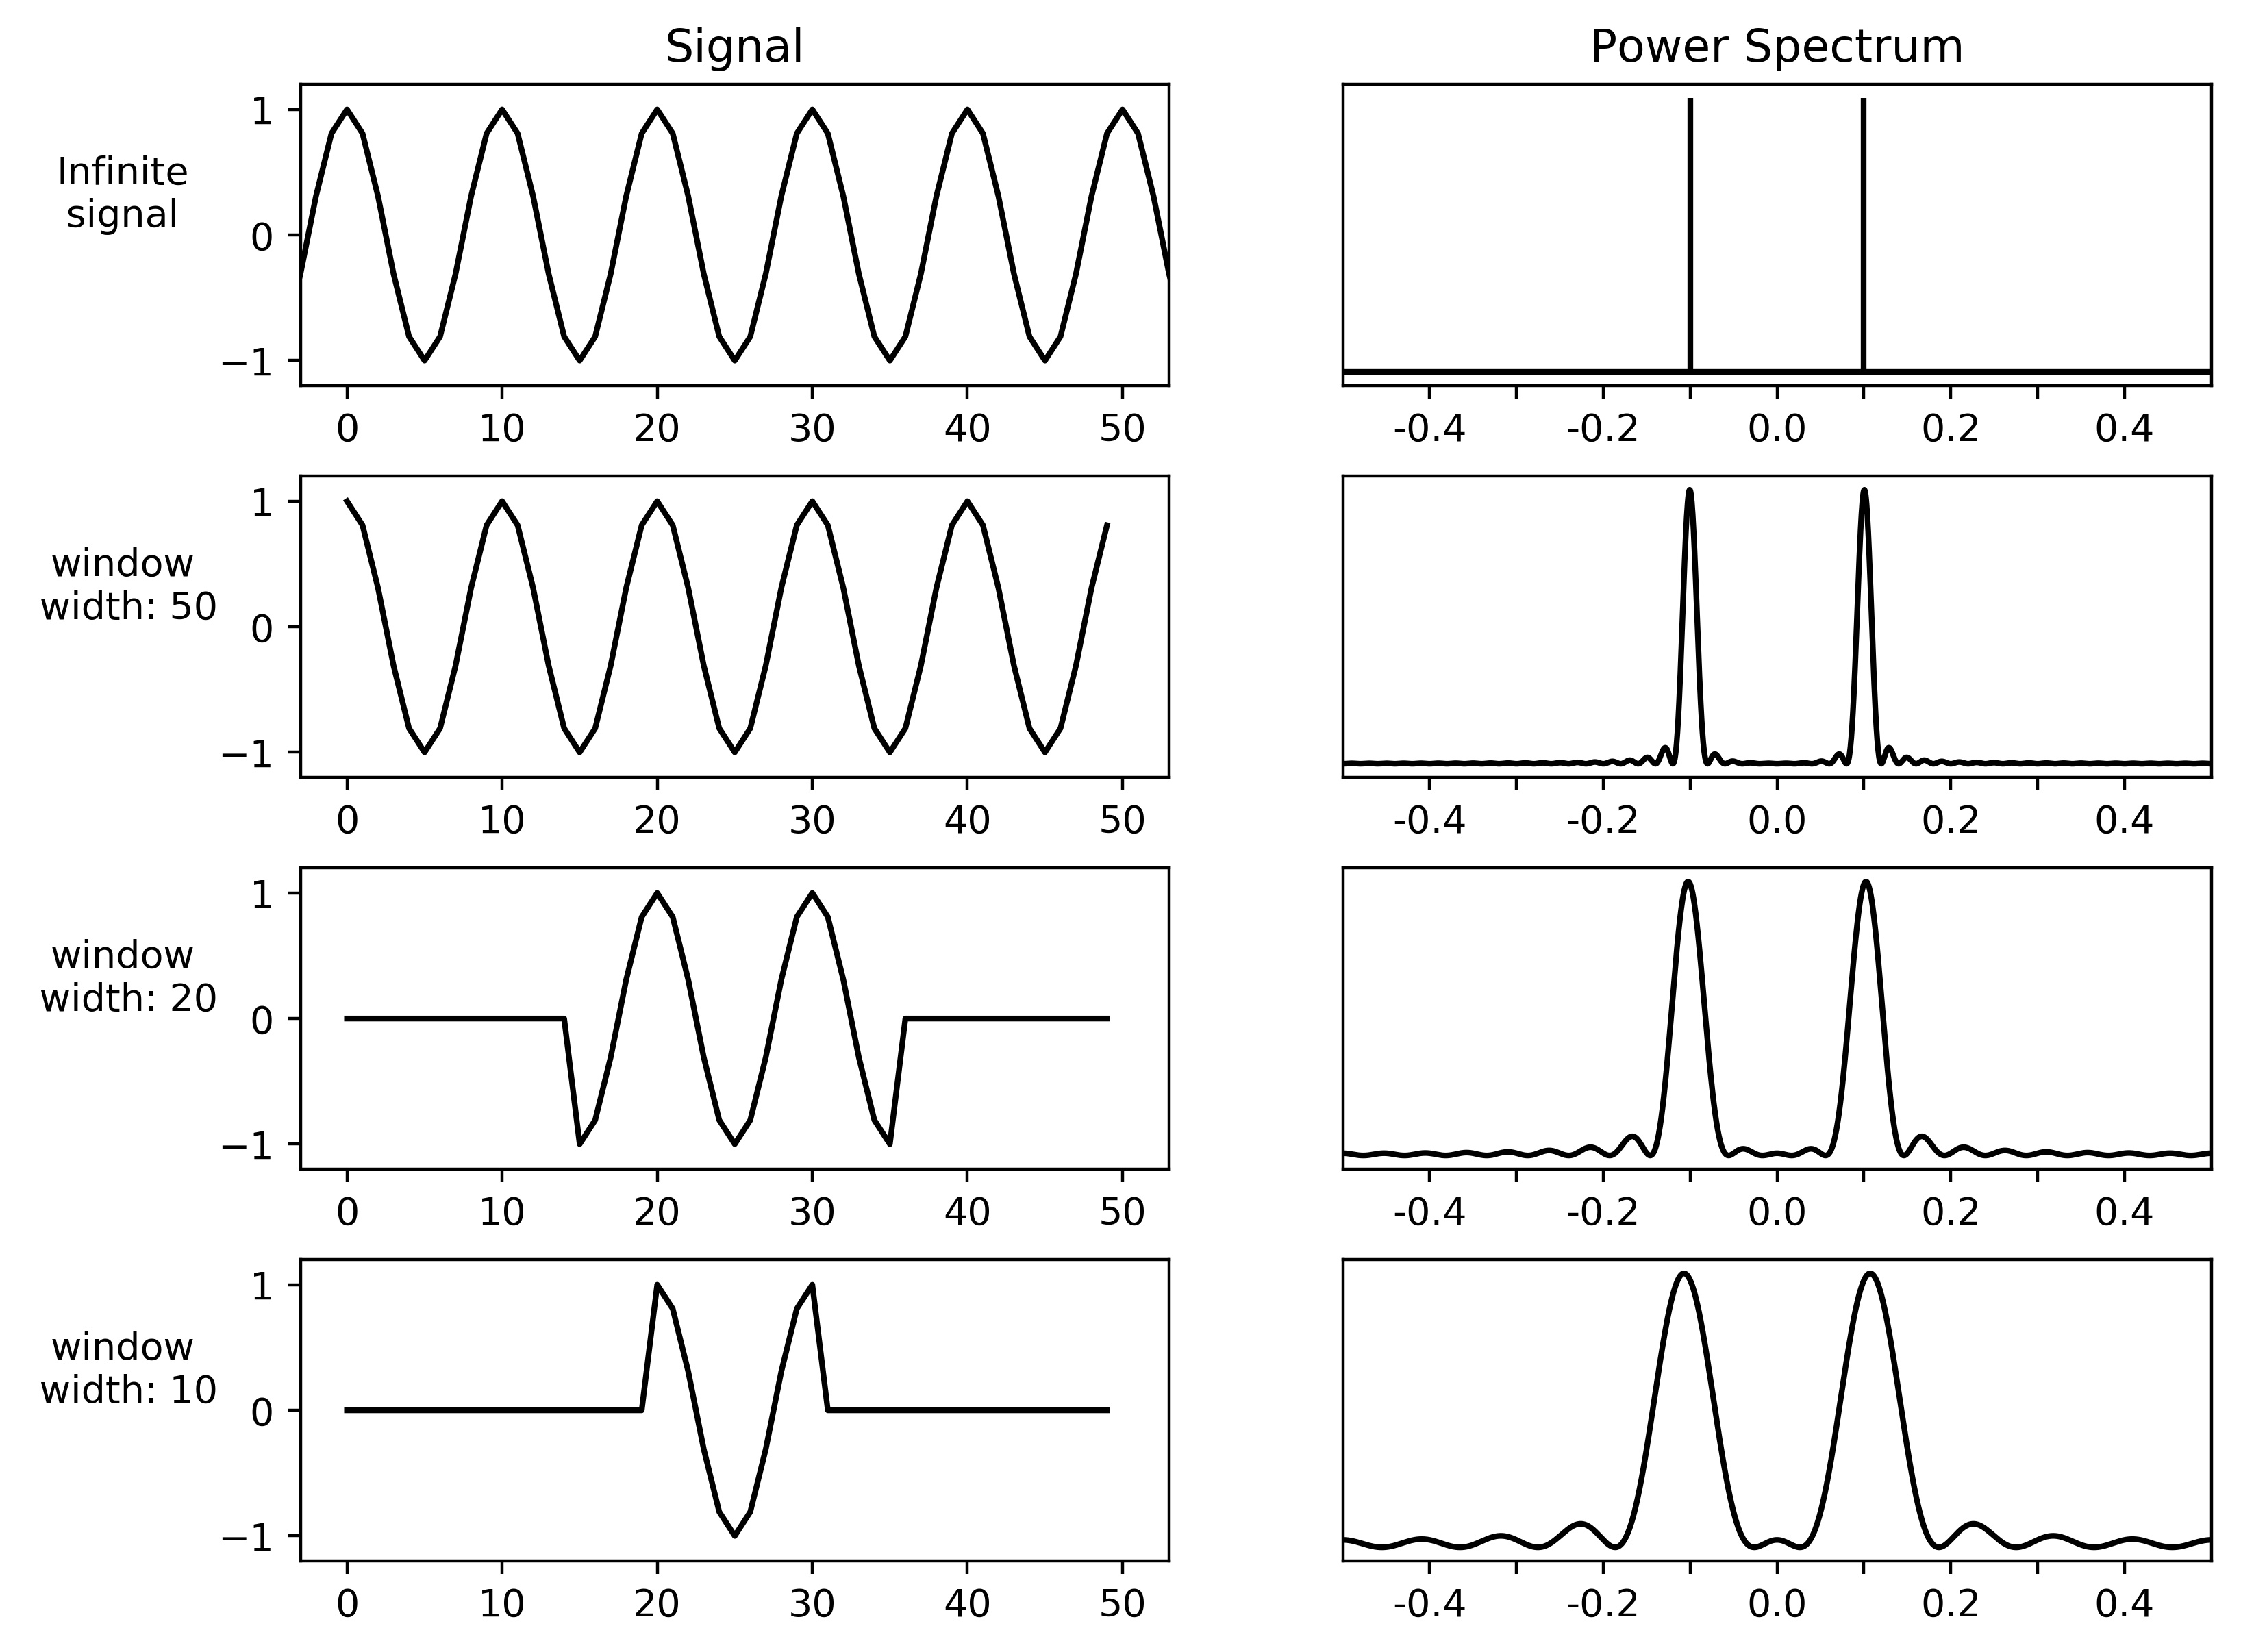
\includegraphics{Figuras/fig1.jpg}}
	\end{center}
	\vspace{1mm}	% acrescentar o espaçamento vertical apropriado entre a borda inferior da figura e a legenda ou a fonte quando não há legenda (o valor pode ser negativo para subir)
	\legenda{Efeitos do tamanho da janela de observação sobre o espectro de potência de um sinal. No topo à esquerda o sinal está representado por uma função analítica que se estende infinitamente, cuja transformada de Fourier (topo à direita) é a função delta sobre a frequência do sinal (no caso, 0.1). Abaixo estão sinais com janelas de observação diferentes e seus respectivos espectros. Quanto menor a janela de observação, maior o efeito dos lóbulos laterais sobre a função delta original, o chamado leakage espectral.}	% legenda - para deixar sem legenda usar comando \legenda{} (nunca deve-se comentar o comando \legenda)
	\label{fig:window}
	%\FONTE{\url{https://omniweb.gsfc.nasa.gov/form/dx1.html}.}	% fonte consultada (elemento obrigatório, mesmo que seja produção do próprio autor)
\end{figure}

\begin{figure}[ht!]
	\caption{Efeitos do sampling rate.}
	\vspace{1mm}	% acrescentar o espaçamento vertical apropriado entre o título e a borda superior da figura
	\begin{center}
		\resizebox{15cm}{!}{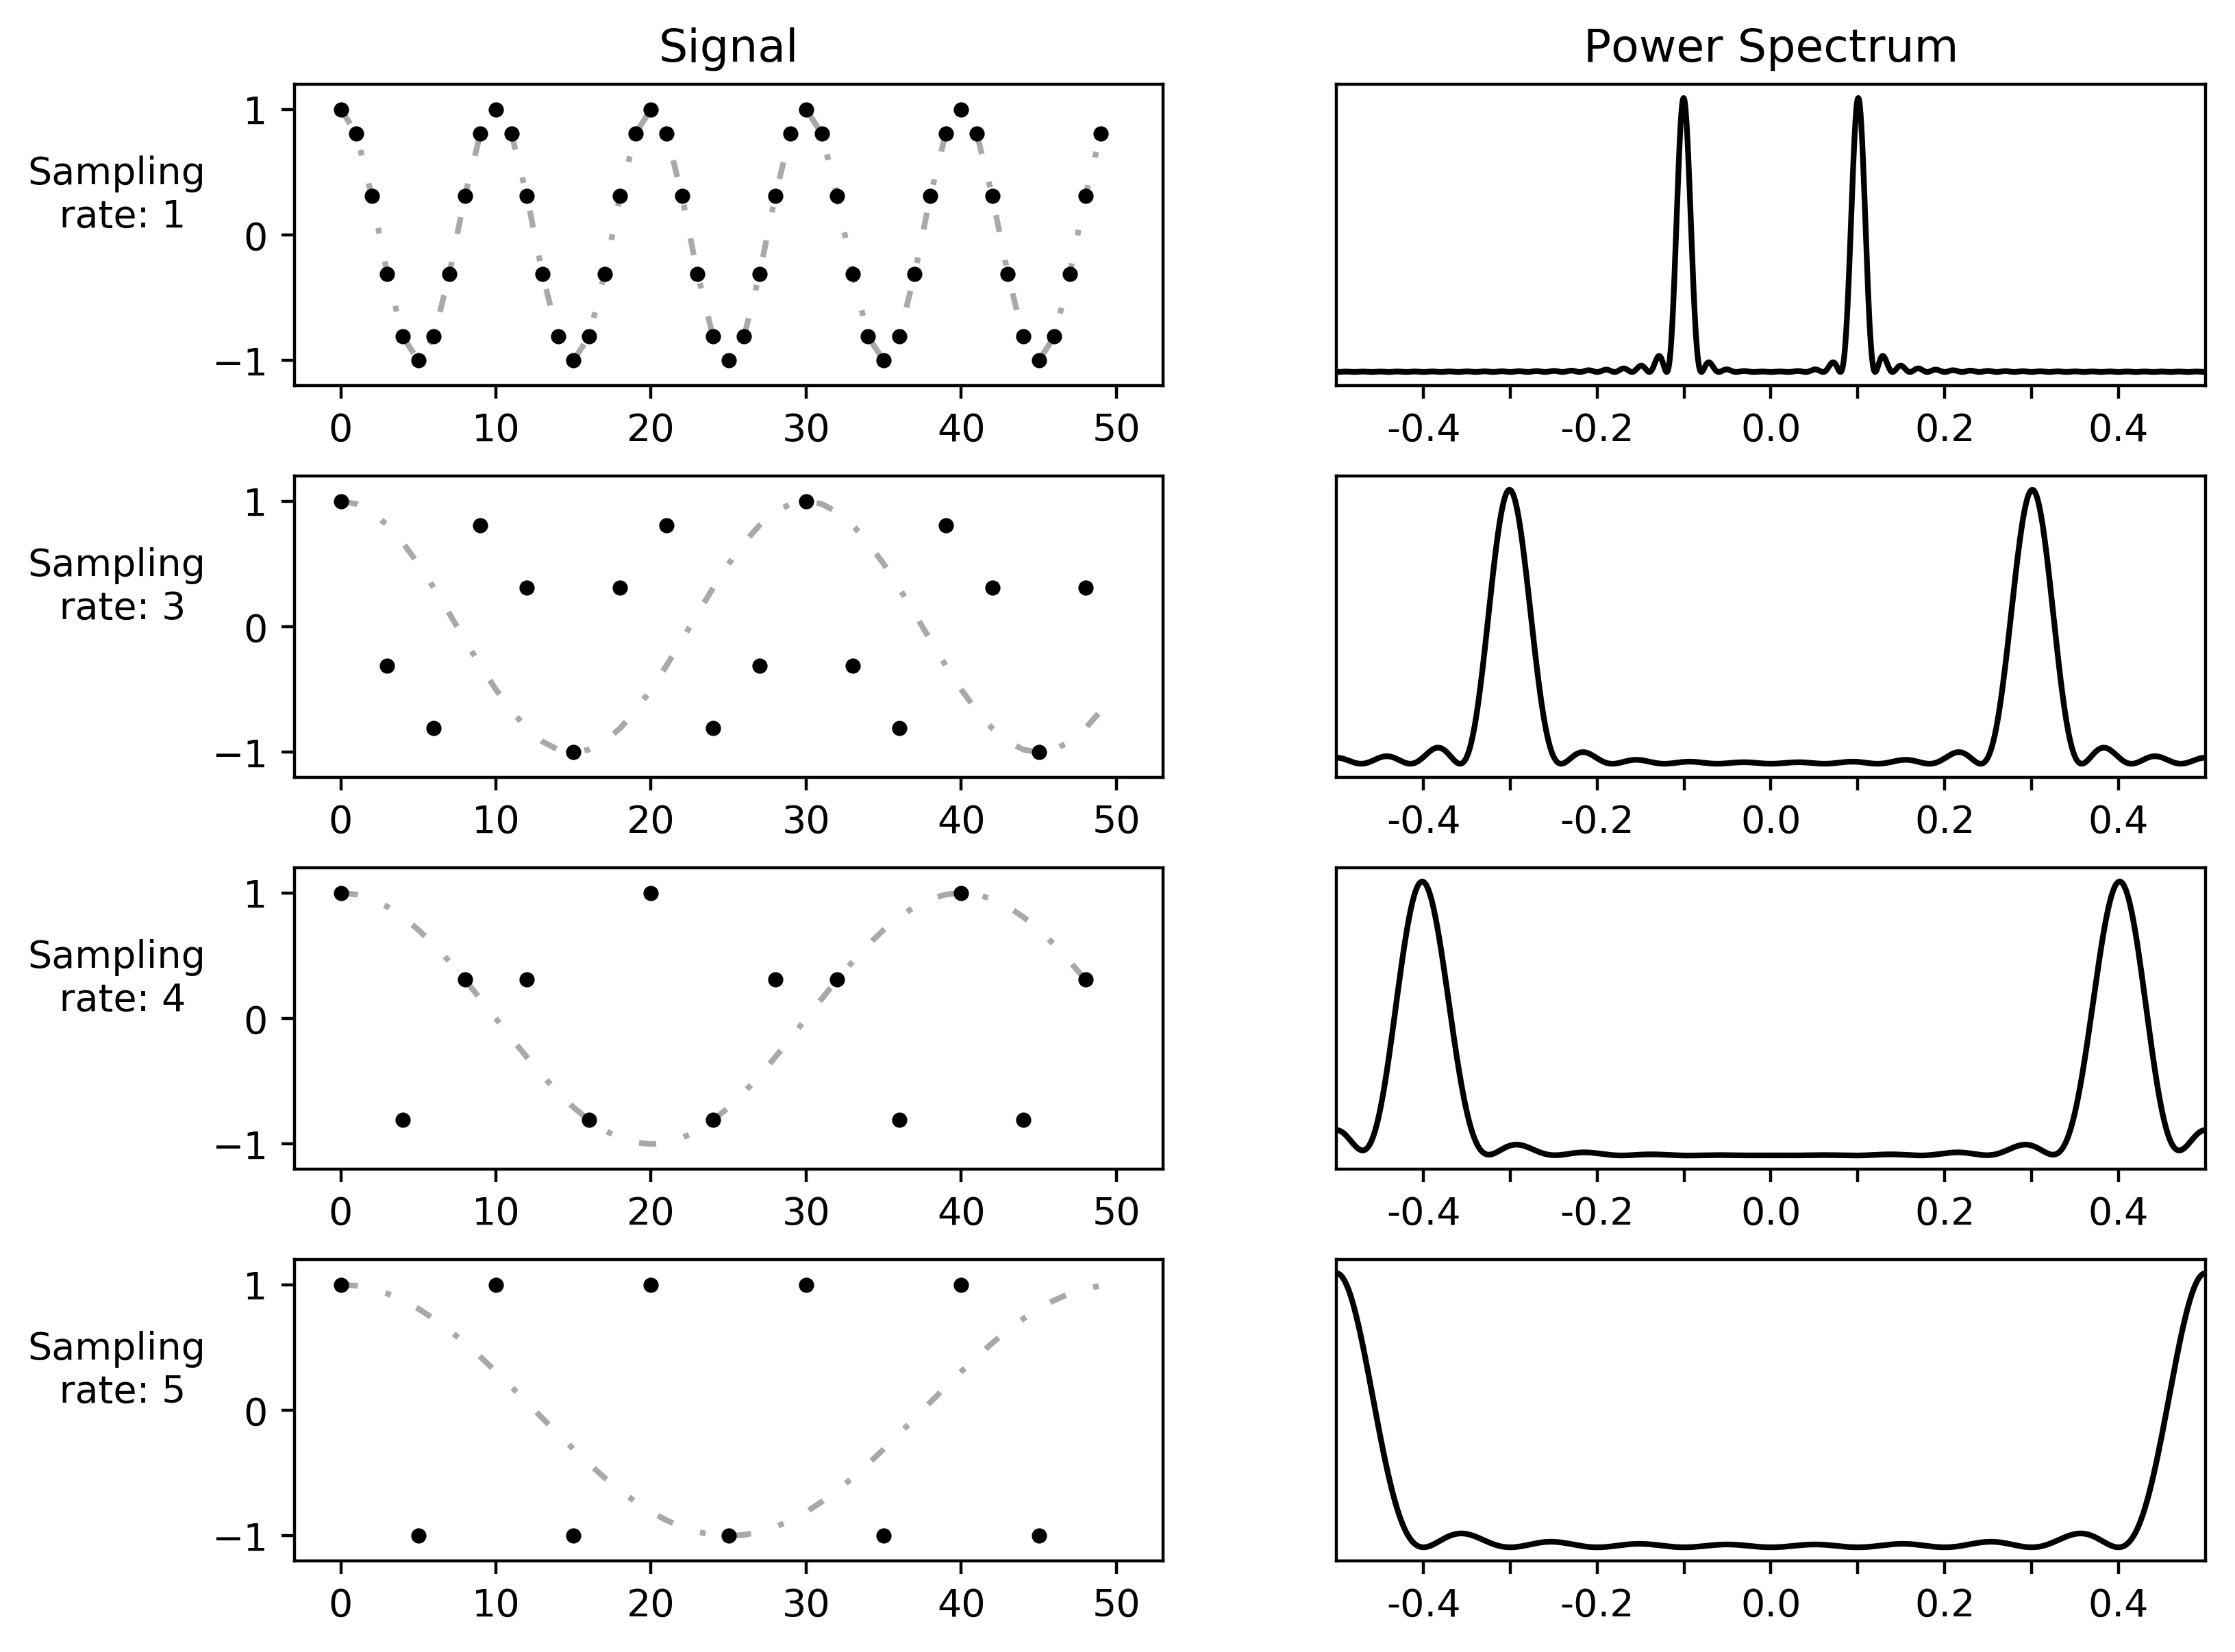
\includegraphics{Figuras/fig2.jpg}}
	\end{center}
	\vspace{1mm}	% acrescentar o espaçamento vertical apropriado entre a borda inferior da figura e a legenda ou a fonte quando não há legenda (o valor pode ser negativo para subir)
	\legenda{Efeitos do sampling rate sobre o espectro de potência de um sinal. No topo, um sinal com um sampling rate igual a um (que corresponde ao sinal com janela de tamanho 50 na Figura \ref{fig:window}). Abaixo, o mesmo sinal sob diferentes sampling rates e seus respectivos espectros. A linha pontilhada/tracejada em cinza claro ilustra o sinal falsamente identificado, tanto pelo nosso cérebro quanto pela FFT, conforme indicado nos seus espectros de potência à direita. Fica evidente que para diferentes taxas, diferentes aliases do sinal original são gerados, de modo que a transformada inversa retornaria um sinal totalmente diferentes do original.} % 	% legenda - para deixar sem legenda usar comando \legenda{} (nunca deve-se comentar o comando \legenda)
	\label{fig:sampling}
	%\FONTE{\url{https://omniweb.gsfc.nasa.gov/form/dx1.html}.}	% fonte consultada (elemento obrigatório, mesmo que seja produção do próprio autor)
\end{figure}

Os lóbulos laterais (leakage spectral) são um artefato devido ao intervalo de observação ser finito. As falsas frequências (aliasing) é uma artefato que surge da natureza do sampling. Sabemos que nossos dados de fluxo solar F10.7 são finitos no tempo e apresentam um sampling rate uniforme e satisfatório para gerar bons espectros via FFT, conforme explicitado em \citeonline{Leo}. Mas qual seria o efeito de sampling não uniforme sobre o sinal das figuras anteriores? A Figura 3 ilustra dois cenários de ausência de dados e seus respectivos espectros. Fica evidente a incrível irregularidade do espectro de potência resultante da FFT devido a um espaçamento desigual da amostragem do sinal. 

\begin{figure}[ht!]
	\caption{Efeitos do sampling não uniforme.}
	\vspace{1mm}	% acrescentar o espaçamento vertical apropriado entre o título e a borda superior da figura
	\begin{center}
		\resizebox{15cm}{!}{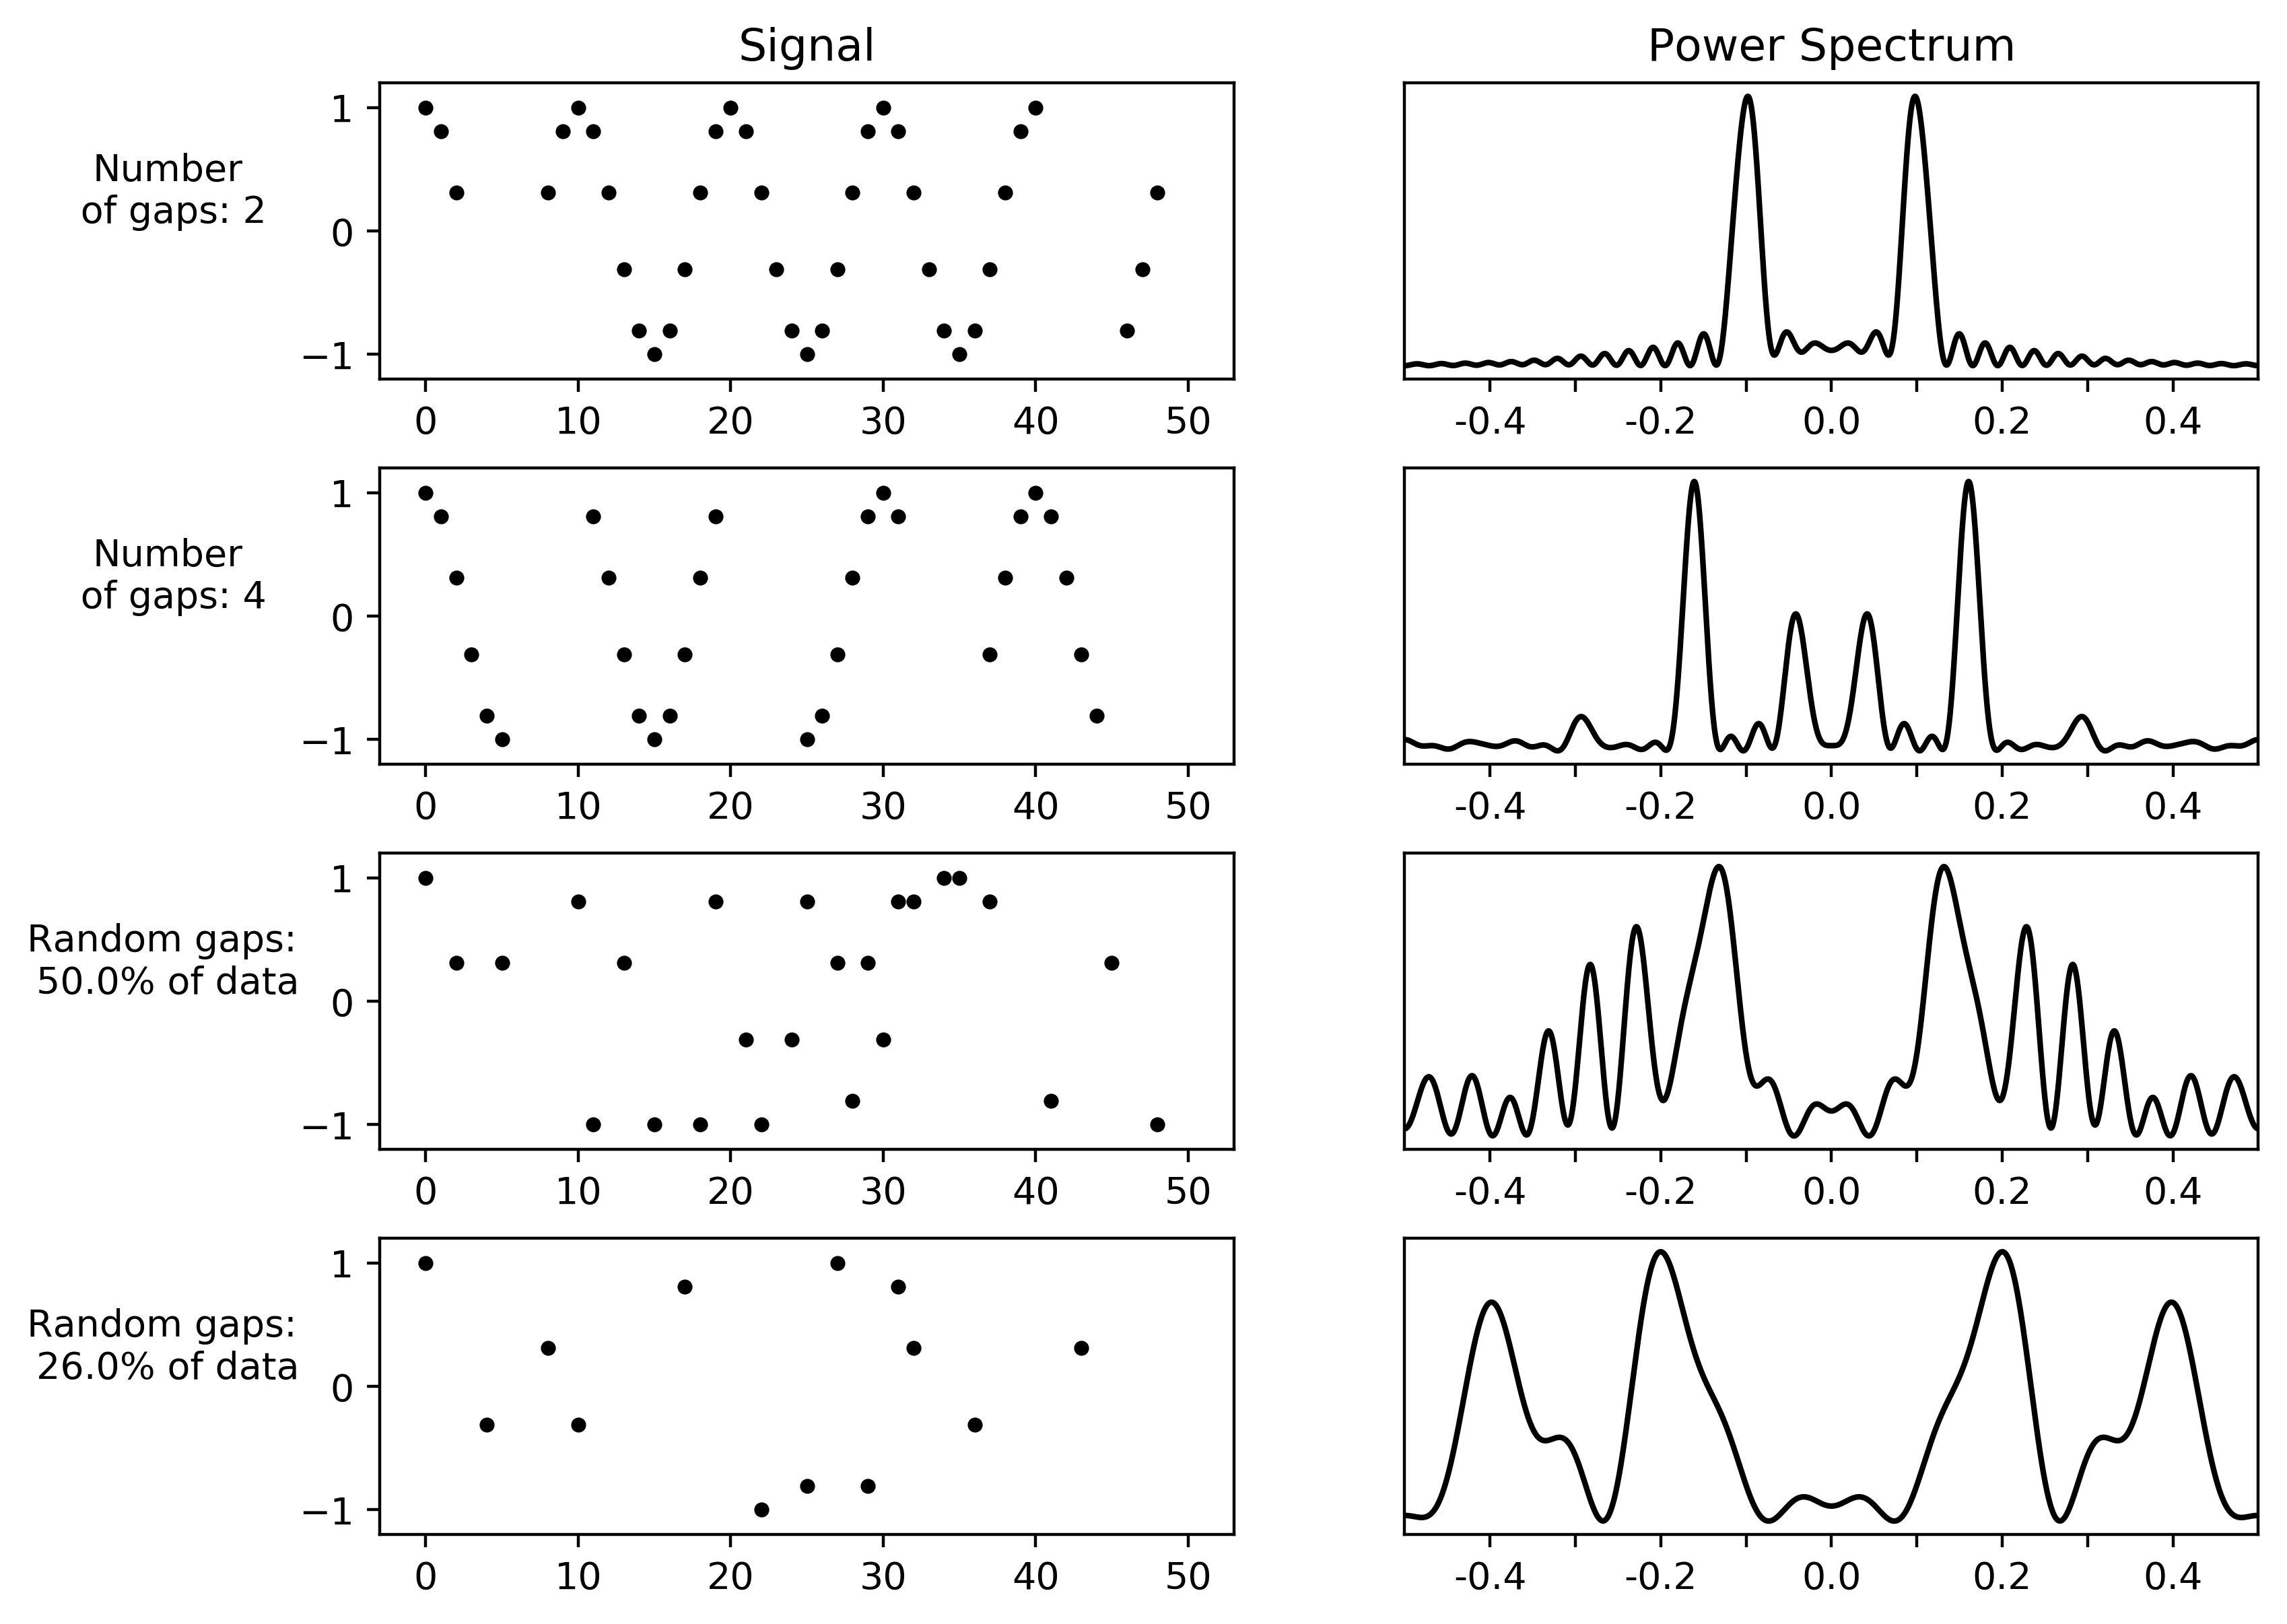
\includegraphics{Figuras/fig3.jpg}}
	\end{center}
	\vspace{1mm}	% acrescentar o espaçamento vertical apropriado entre a borda inferior da figura e a legenda ou a fonte quando não há legenda (o valor pode ser negativo para subir)
	\legenda{Efeitos do sampling não uniforme sobre o espectro de potência de um sinal. No topo, o sinal do topo da Figura \ref{fig:window} se apresenta com dois gaps (intervalos) aleatórios sem dados. Abaixo deste, o mesmo sinal com quatro gaps aleatoriamente posicionados. Os dois últimos sinais representam um cenário com remoção aleatória de dados, um permanecendo com 50\% dos dados e o outro com 26\% apenas. Somente o espectro de potência do primeiro sinal (topo à direita) possui um pico consistente (posicionado na frequência esperada de 0.1).}	% legenda - para deixar sem legenda usar comando \legenda{} (nunca deve-se comentar o comando \legenda)
	\label{fig:uneven}
	%\FONTE{\url{https://omniweb.gsfc.nasa.gov/form/dx1.html}.}	% fonte consultada (elemento obrigatório, mesmo que seja produção do próprio autor)
\end{figure}


\section{Periodograma de Lomb-Scargle}

O periodograma de Lomb-Scargle é a principal ferramenta para análise de séries temporais com amostragem desigual. Ele pertence a um grupo de ferramentas de análise espectral que explora o método de mínimos quadrados, estimando frequências do sinal a partir de testes sobre frequências pré-determinadas com o fim de ajustar funções senoidais aos dados. O periodograma de Lomb-Scargle é dos métodos de análise espectral por mínimos quadrados desenvolvido por \citeonline{lomb1976least} com posterior contribuição de \citeonline{scargle1982studies}. Ele está disponível no pacote \texttt{astropy} (com complexidade $O[NlogN]$) através da classe \texttt{LombScargle}, e pode ser facilmente implementado:

\vspace{-2mm}
\begin{lstlisting}[language=python,style=mystyle2]
from astropy.timeseries import LombScargle
frequency, power = LombScargle(t, f).autopower()
\end{lstlisting}

No exemplo acima, o periodograma de Lomb-Scargle foi aplicado a um sinal \texttt{f} amostrado em tempos irregulares conforme o array \texttt{t}, gerando um array com as frequências testadas (\texttt{frequency}) e o periodograma resultante (\texttt{power}). O método \texttt{autopower()} aplica uma heurística para selecionar frequências adequadas ao teste de mínimos quadrados. Pode-se ajustar essa mesma heurística para testar frequências mais altas e com maior resolução através da palavra-chave \texttt{nyquist\_factor}. O valor de dois foi empregado nas análises deste trabalho. Além disso, é possível passar como um terceiro input a incerteza dos dados, pois a classe \texttt{LombScargle} é capaz de considerar incertezas em seus cálculos (assume-se incerteza gaussiana). O sinusoide de melhor ajuste pode ser computado a partir do método \texttt{model()}. O output da classe \texttt{LombScargle} é adimensional e por padrão normalizado (seus valores estão entre 0 e 1). Alguns desses recursos são explorados na próxima seção.

%\begin{lstlisting}[language=python,style=mystyle2]
%frequency,power=LombScargle(t,y,dy).autopower(nyquist_factor=10)
%\end{lstlisting}

%A seção a seguir apresenta o resultado da implementação desta classe sobre diferentes cenários de aquisição aleatória dos dados de fluxo solar F10.7.  

